\newpage
\section{TEM}

 Es wird ein Libra 200 FE TEM (Zeiss) verwendet, um die in \cref{sec:prep} beschriebenen Proben zu untersuchen.
 Hierbei zeigt sich, dass die durchschnittlich etwa \SI{20}{nm} großen Goldcluster aufgelöst werden können.
 Aufgrund von Problemen mit dem Gerät werden jedoch im Folgenden ältere Messungen von Wolframdiselenid ausgewertet.

 In \cref{fig:tem_dfbf} sind hiermit aufgenommene Hell- und Dunkelfeldbilder dargestellt.
 Für die Hellfeldaufnahme wird in der Streuebene mittels einer Blende alle Strahlen außer des ungestreuten Elektronenstrahls herausgefiltert.
 Dementsprechend werden dickere Strukturen im Bild dunkel sichtbar, während dünne Strukturen heller und Orte ohne Probe am hellsten erscheinen.

 Für die Dunkelfeldaufnahme wird stattdessen einer der gebeugten Spots in der Streuebene ausgewählt.
 Hierdurch erscheinen besonders stark streuende, also dicke, Strukturen heller.

	\begin{figure}[H]
		\centering
	\begin{subfigure}[b]{0.45\textwidth}
				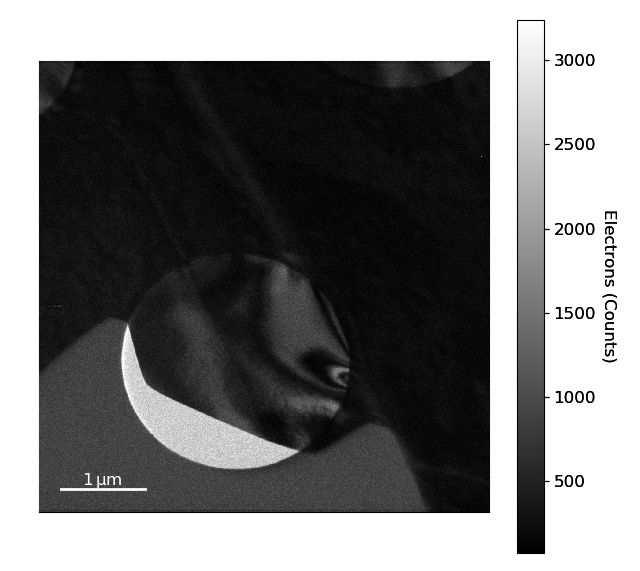
\includegraphics[width= 1 \linewidth]{img/tem_bf}
				\caption{Hellfeld}
		\end{subfigure}
	\begin{subfigure}[b]{0.45\textwidth}
				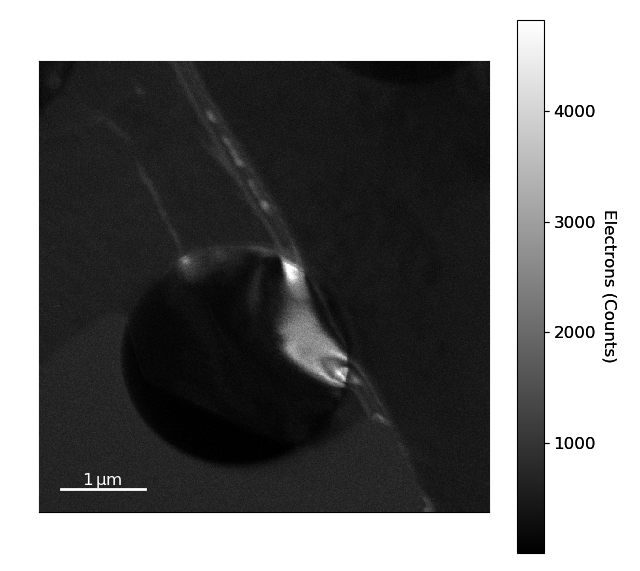
\includegraphics[width= 1 \linewidth]{img/tem_df}
				\caption{Dunkelfeld}
		\end{subfigure}
		\caption{
      Hell- und Dunkelfeld-Aufnahmen im TEM. Die runde Form ist ein Loch im membranartigen Probenhalter. Im Hellfeld ist der WSe$_2$-Kristall über dem Loch in dunkler Farbe erkennbar. Im Dunkelfeld ist in heller Farbe sichtbar, wo der Kristall besonders dick ist.
				}
    \label{fig:tem_dfbf}
	\end{figure}



 \subsection{Bestimmung der Atomabstände in der Projektionsebene}

 In \cref{fig:hrtem} ist die Aufnahme der Oberfläche des Kristalls dargestellt.
 Daraus werden durch Abzählen der Täler im Linienprofil die Atomabstände in den beiden sichtbaren Richtungen bestimmt und in \cref{tab:netz} dargestellt.
 Die Unsicherheit wurde mit einer Abweichung in Höhe von einem Atomabstand über die abgezählte Täler abgeschätzt.

	\begin{figure}[H]
		\centering
	\begin{subfigure}[b]{0.40\textwidth}
        \centering
				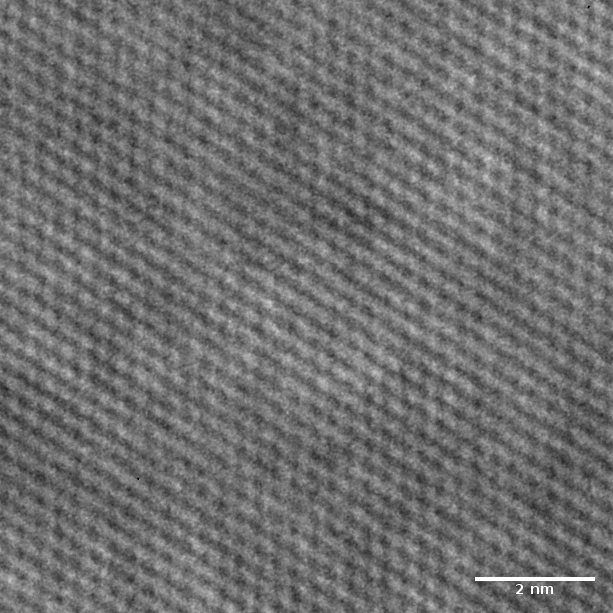
\includegraphics[width= 1 \linewidth]{img/hrtem_zoomzoom}
				\caption{}
        \label{fig:hrtem_img}
		\end{subfigure}

	\begin{subfigure}[b]{0.65\textwidth}
        \centering
				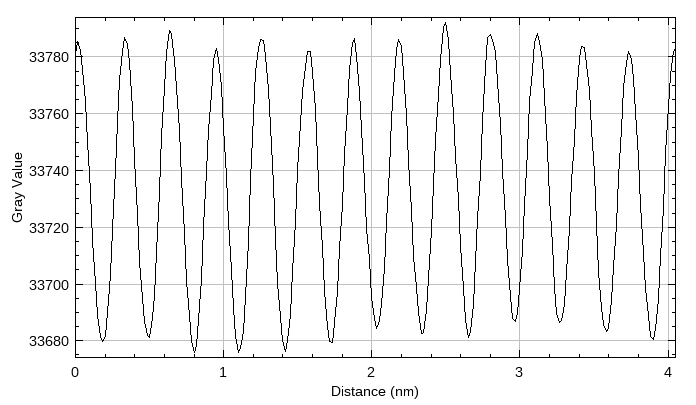
\includegraphics[width= 1 \linewidth]{img/tem_line-Plot_hrtem_orig}
				\caption{}
		\end{subfigure}
		\caption{
      TEM-Aufnahme der Oberfläche des WSe$_2$-Kristalls und eines der Linienprofile. Für dieses wurde über mehrere parallele Atomreihen gemittelt, wodurch das Rauschen stark verringert wurde.
				}
    \label{fig:hrtem}
	\end{figure}

  Für \cref{fig:ft} wurde diese Aufnahme (mit geringerer Vergrößerung als in \cref{fig:hrtem_img}) fouriertransformiert.
  Darin tauchen räumliche Frequenzen (die Gitterstruktur) als helle Punkte auf.
  Aus der Position dieser Punkte ergibt sich die räumliche Wellenlänge, die hier dem Atomabstand entspricht.
  Die so ermittelten Atomabstände sind in \cref{tab:netz} eingetragen.
  Für die Unsicherheit wurde die FWHM der räumlichen Peaks verwendet.

	\begin{figure}[H]
  \centering
			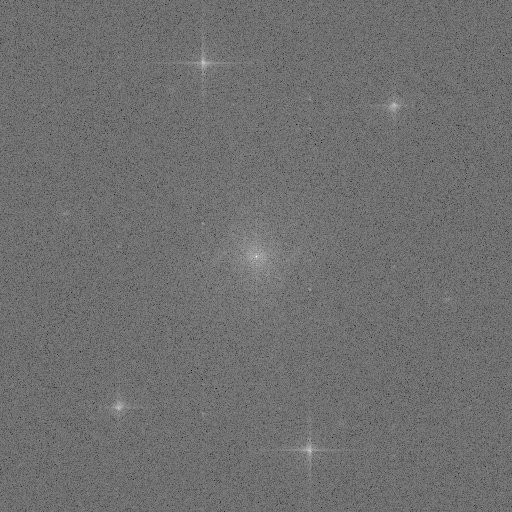
\includegraphics[width= 0.4 \linewidth]{img/tem_hrtem_crop_fft}
			\caption{
        Räumliche Fouriertransformation der TEM-Aufnahme in \cref{fig:hrtem}.
			}
			\label{fig:ft}
	\end{figure}

  Als letzte Methode wird das Bild in der Streuebene bei Beleuchtung einer hinreichend großen Fläche (einige Atomabstände) aufgenommen und in \cref{fig:diff} abgebildet.
  Anhand der Abstände der Spots werden über den Kehrwert die Atomabstände des Realraumgitters (in der Projektion auf eine Ebene) bestimmt und in \cref{tab:netz} vermerkt.
  Es wird der Abstand über mehrere Spots gemessen und gemittelt.

	\begin{figure}[H]
  \centering
			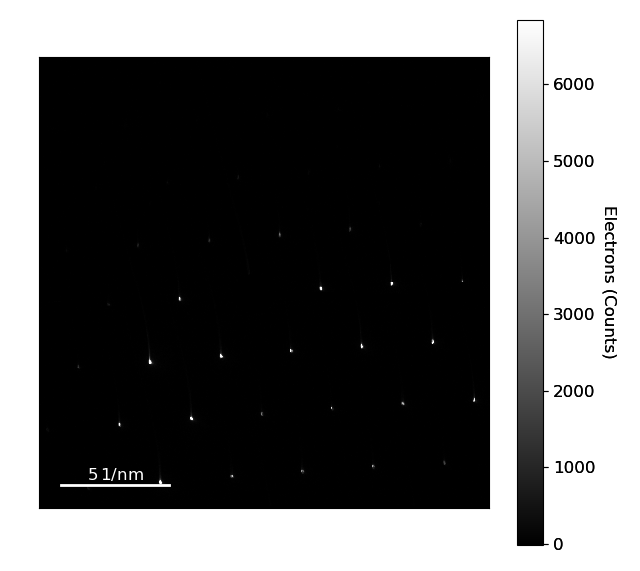
\includegraphics[width= 0.6 \linewidth]{img/tem_diff}
			\caption{
        TEM-Aufnahme in der Streuebene.
			}
			\label{fig:diff}
	\end{figure}



	\begin{table}
		\centering
		\caption{Auf unterschiedliche Arten bestimmte Atomabstände der WSe$_2$-Probe. Die Richtungen können sind nur zu Unterscheidung innerhalb der selben Messmethode angegeben. Zwischen den Methoden sind die Richtungen nicht konstant.
    Für den Literaturwert wurde der Abstand zwischen den Selenatomen angegeben.}
		\begin{tabular}{c| c | c}
			Methode & Richtung & Atomabstand \\ \hline
			% & & & \\
      Linienprofil &  1 & \SI{0.31 \pm 0.01}{nm}\\
      Linienprofil &  2 & \SI{0.31 \pm 0.01}{nm}\\
      Fouriertransformation & 1 & \SI{0.29 \pm 0.01}{nm}\\
      & 2 & \SI{0.3 \pm 0.01}{nm}\\
      Streuebene & 1 & \SI{0,312 \pm 0.001}{nm} \\
      & 2 & \SI{0,317 \pm 0.001}{nm} \\
      & 3 & \SI{0,314 \pm 0.001}{nm} \\
      Mittelwert & & \SI{0,308 \pm 0.002}{nm}\\
      Literatur & & \SI{0,334}{nm} \cite{wiki_wse}\\
		\end{tabular}
		\label{tab:netz}
	\end{table}

\subsection{Diskussion der TEM-Ergebnisse}

  Die mittels der verschiedenen Messmethoden ermittelten Atomabstände in \cref{tab:netz} stimmen innerhalb der Messunsicherheit miteinander überein.
  Dass abhängig von der Messrichtung kein Unterschied im Atomabstand besteht, stimmt mit der zu erwartenden hexagonalen Symmetrie innerhalb einer Wolframdiselenidlage überein.
  Die Abweichung nach Unten gegenüber dem Literaturwert für den Abstand der Selenatome kommt dadurch zustande, dass nicht dieser Abstand, sondern der Abstand der Projektion der Atome (Wolfram und Selen) auf eine ebene Fläche gemessen wurde.
  Wie in \cref{fig:strukt} zu sehen ist, liegen auch innerhalb einer Monolage nicht alle Atome in einer Ebene.

	\begin{figure}[H]
  \centering
			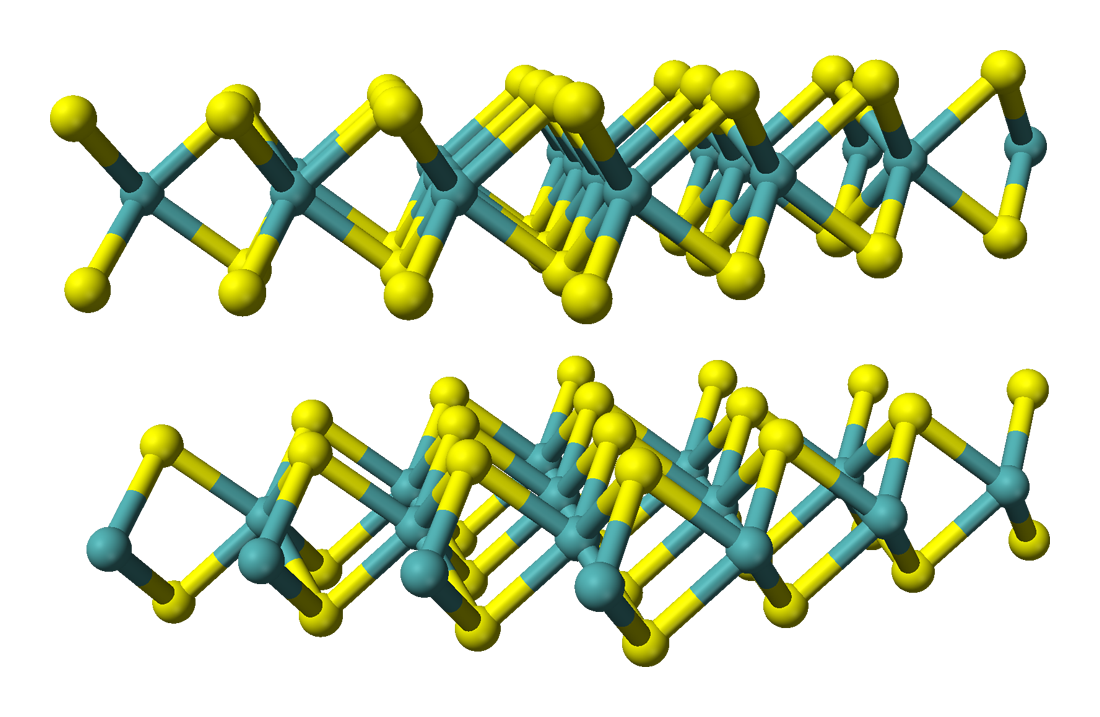
\includegraphics[width= 0.4 \linewidth]{img/strukt}
			\caption{
        Struktur einer Monolage Wolframdiselenid. \cite{wiki_wse_bild}
			}
			\label{fig:strukt}
	\end{figure}

  \subsection{EELS}

	\begin{figure}[H]
		\centering
	\begin{subfigure}[b]{0.45\textwidth}
				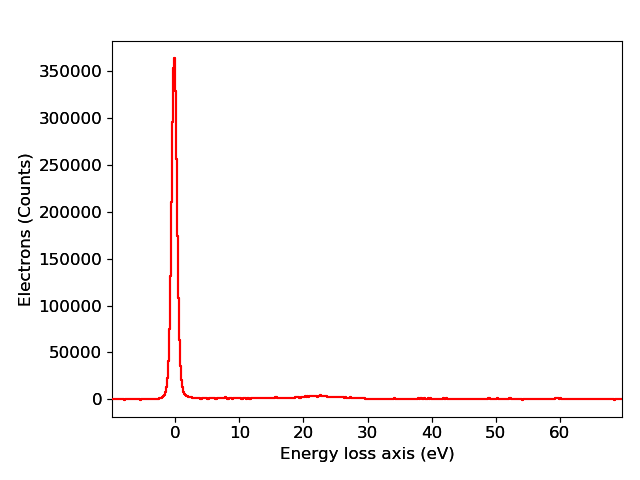
\includegraphics[width= 1 \linewidth]{img/tem_zeroloss}
				\caption{zero-loss}
	\end{subfigure}
	\begin{subfigure}[b]{0.45\textwidth}
				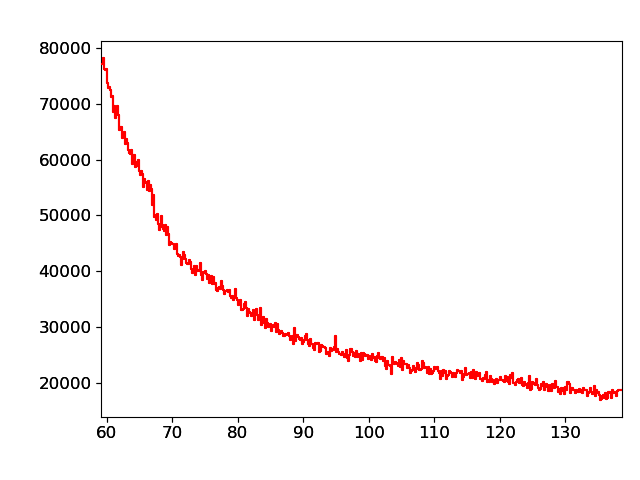
\includegraphics[width= 1 \linewidth]{img/tem_coreloss}
				\caption{core-loss}
	\end{subfigure}
	\begin{subfigure}[b]{0.7\textwidth}
				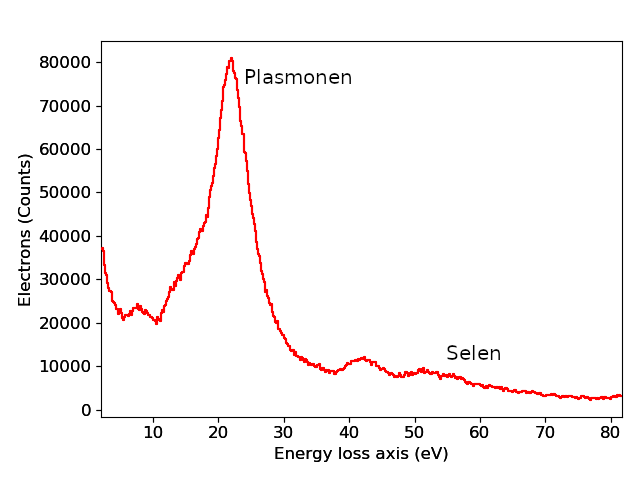
\includegraphics[width= 1 \linewidth]{img/tem_mark}
				\caption{low-loss}
	\end{subfigure}
		\caption{
      EELS-Spektren der Wolframdiselenidprobe.
			}
    \label{fig:eels}
	\end{figure}

  Zuletzt wird das EEL-Spektrum der Probe aufgenommen.
  Es ist in \cref{fig:eels} zu sehen.
  Hier wurden die deutlich erkennbaren Peaks entsprechend ihres Ursprungs beschriftet.
  Wolfram hat lediglich Kanten im Bereich von über \SI{1800}{eV}, also außerhalb des Messbereichs, und eine O-Kante bei \SI{36}{eV} \cite{eelsinfo}, die jedoch im Spektrum aufgrund ihrer geringen Intensität und hohen Ausgeschmiertheit nicht zu erkennen ist.

  Selen besitzt zwei Kanten über \SI{1400}{eV}, die ebenfalls nicht mehr im Messbereich sind.
  Die M$_{4,5}$-Kante bei \SI{57}{eV} ist jedoch erkennbar.

  Außerdem ist der Plasmonenpeak im Low-Loss-Bereich zu erkennen.
  Im Core-Loss-Bereich sind keine Peaks sichtbar, was anhand der für Wolfram und Selen auf Basis von \cite{eelsinfo} bekannten Kanten der Erwartung entspricht.


 %die Multimap-Dateien sind EFTEM-Aufnahmen. Da sollen wir denke nichts mit machen
